\documentclass[10pt,letterpaper]{article}
% Add a bunch of useful math, font, and symbols
\usepackage{amsfonts}
\usepackage{amsmath}
\usepackage{amssymb}

% English support
\usepackage[english]{babel}

% Citation
\usepackage[superscript]{cite}

% Better enumerate and itemize
\usepackage{enumitem}

% Better control of headers and footers
\usepackage{fancyhdr}

% Floating objects like figures and tables
\usepackage{float}

% Page layout and dimensioning
\usepackage[margin=1in]{geometry}

% Basic color, graphics and text manipulation 
\usepackage{graphicx}

% Use Helvetica typeface
\usepackage[scaled]{helvet}
\renewcommand\familydefault{\sfdefault} 
\usepackage[T1]{fontenc}

% Cross-referencing hyperlinks
\usepackage{hyperref}

% Line break for long URLs
\usepackage{breakurl}

% Accept utf-8 input encoding
\usepackage[utf8]{inputenc}

% Make indexes
\usepackage{makeidx}

% Microtype (apparently makes the typographics stuff better)
\usepackage{microtype}

% [Disabled] multi-column writing
% \usepackage{multicol}

% English ordinal counting (1st, 2nd, etc.)
\usepackage{nth}

% Long table
\usepackage{longtable}

% Paragraph skip - adds extra lineskip spacing
\usepackage{parskip}
\setlength{\parskip}{0.7\baselineskip plus 2pt}

% Add ability to set space between lines
\usepackage{setspace}

% S.I. units
\usepackage{siunitx}

% Subcaptions for subfigures
\usepackage{subcaption}

% Include svg graphics
\usepackage{svg}

% Drawing graphics
\usepackage{tikz}

% Subsubsubsection
\usepackage{titlesec}
\setcounter{secnumdepth}{4}
\titleformat{\paragraph}
{\normalfont\normalsize\bfseries}{\theparagraph}{1em}{}
\titlespacing*{\paragraph}
{0pt}{3.25ex plus 1ex minus .2ex}{1.5ex plus .2ex}

% Custom titles
\usepackage{titling}

% Url
\usepackage{url}

\RequirePackage[figure,table]{totalcount}


% Custom definitions
\newcommand{\doctitle}{Operations, Maintenance, and Upgrades Specification}
\newcommand{\docsubtitle}{Computing Platform Multirotor with FPGA Hardware Acceleration Applications}
% Custom commands
\newcommand{\ts}{\textsubscript}	% Subscript command %


\renewcommand{\revisionnum}{1.2}

% Use hyphans to break up urls
\def\UrlBreaks{\do\/\do-}

% PDF and href setup
% Hyper ref
\hypersetup{
	colorlinks=true,
	citecolor=black,
	linkcolor=black,
	filecolor=black,
	urlcolor=blue,
	pdftitle={\@title},
	bookmarks=true
}
\urlstyle{same}
% Page headings
\pagestyle{fancy}
\fancyhead[L]{\MakeUppercase{CPEN/ELEC 491}}
\fancyhead[C]{\textbf{\doctitle}}
\fancyhead[R]{Mieszko Lis, PhD}
\fancyfoot{}
\fancyfoot[C]{Non-Confidential}
\fancyfoot[R]{\thepage}

% No paragraph indent
\parindent 0ex

% Meta
\author{
	Deutsch, Peter &
	\textit{me@peterdeutsch.ca}
	\\
	He, Muchen &
	\textit{m.he@alumni.ubc.ca}
	\\
	Hsueh, Arthur &
	\textit{ah11962@outlook.com}
	\\
	Wang, Meng &
	\textit{wzfftxwd@gmail.com}
	\\
	Wilson, Ardell &
	\textit{ardellw96@gmail.com}
}
\title{\doctitle}
\date{\today}
\makeatletter
\renewcommand{\maketitle}{
	\bgroup
	\setlength{\parindent}{0pt}
	\begin{flushleft}
		% Top spacing
		\vspace*{0.5in}

		% Team logo
		
\includegraphics[scale=0.4]{../assets/capstonelogo1.png}
		\vspace*{0.25in}

		% Title
		\textbf{\Huge{\@title}}\\
		\hrulefill

		% Subtitle
		\textbf{\huge{\docsubtitle}}
		
		\vspace*{0.5in}

		% Course number and team
		\textbf{\Large{CPEN/ELEC 491 Capstone Team 109}}\\
		\hspace*{0.1cm}
		\begin{tabular}[h]{|ll}
			\@author
		\end{tabular}

		\vspace*{0.25in}

		\textbf{\Large{Mieszko Lis, PhD}}\\
		\hspace*{0.1cm}
		\begin{tabular}[h]{|ll}
			Electrical and Computer Engineering, The University of British Columbia
		\end{tabular}

		\vfill
		
		% Date
		\large{Revision 1.0 -- \@date}
		\vspace*{0.5in}

		% Logo
		\hspace*{-0.3cm}
\includegraphics[scale=0.5]{../assets/ece_logo.pdf}

	\end{flushleft}
	\egroup
}
\makeatother

% Begin Document
\begin{document}

% Title Page
\begin{titlepage}
	\maketitle
\end{titlepage}


\renewcommand{\thepage}{\roman{page}}
\setcounter{page}{1}

% Revision history
\backgroundsetup{
	scale=1,
	color=black,
	opacity=0.3,
	angle=0,
	contents={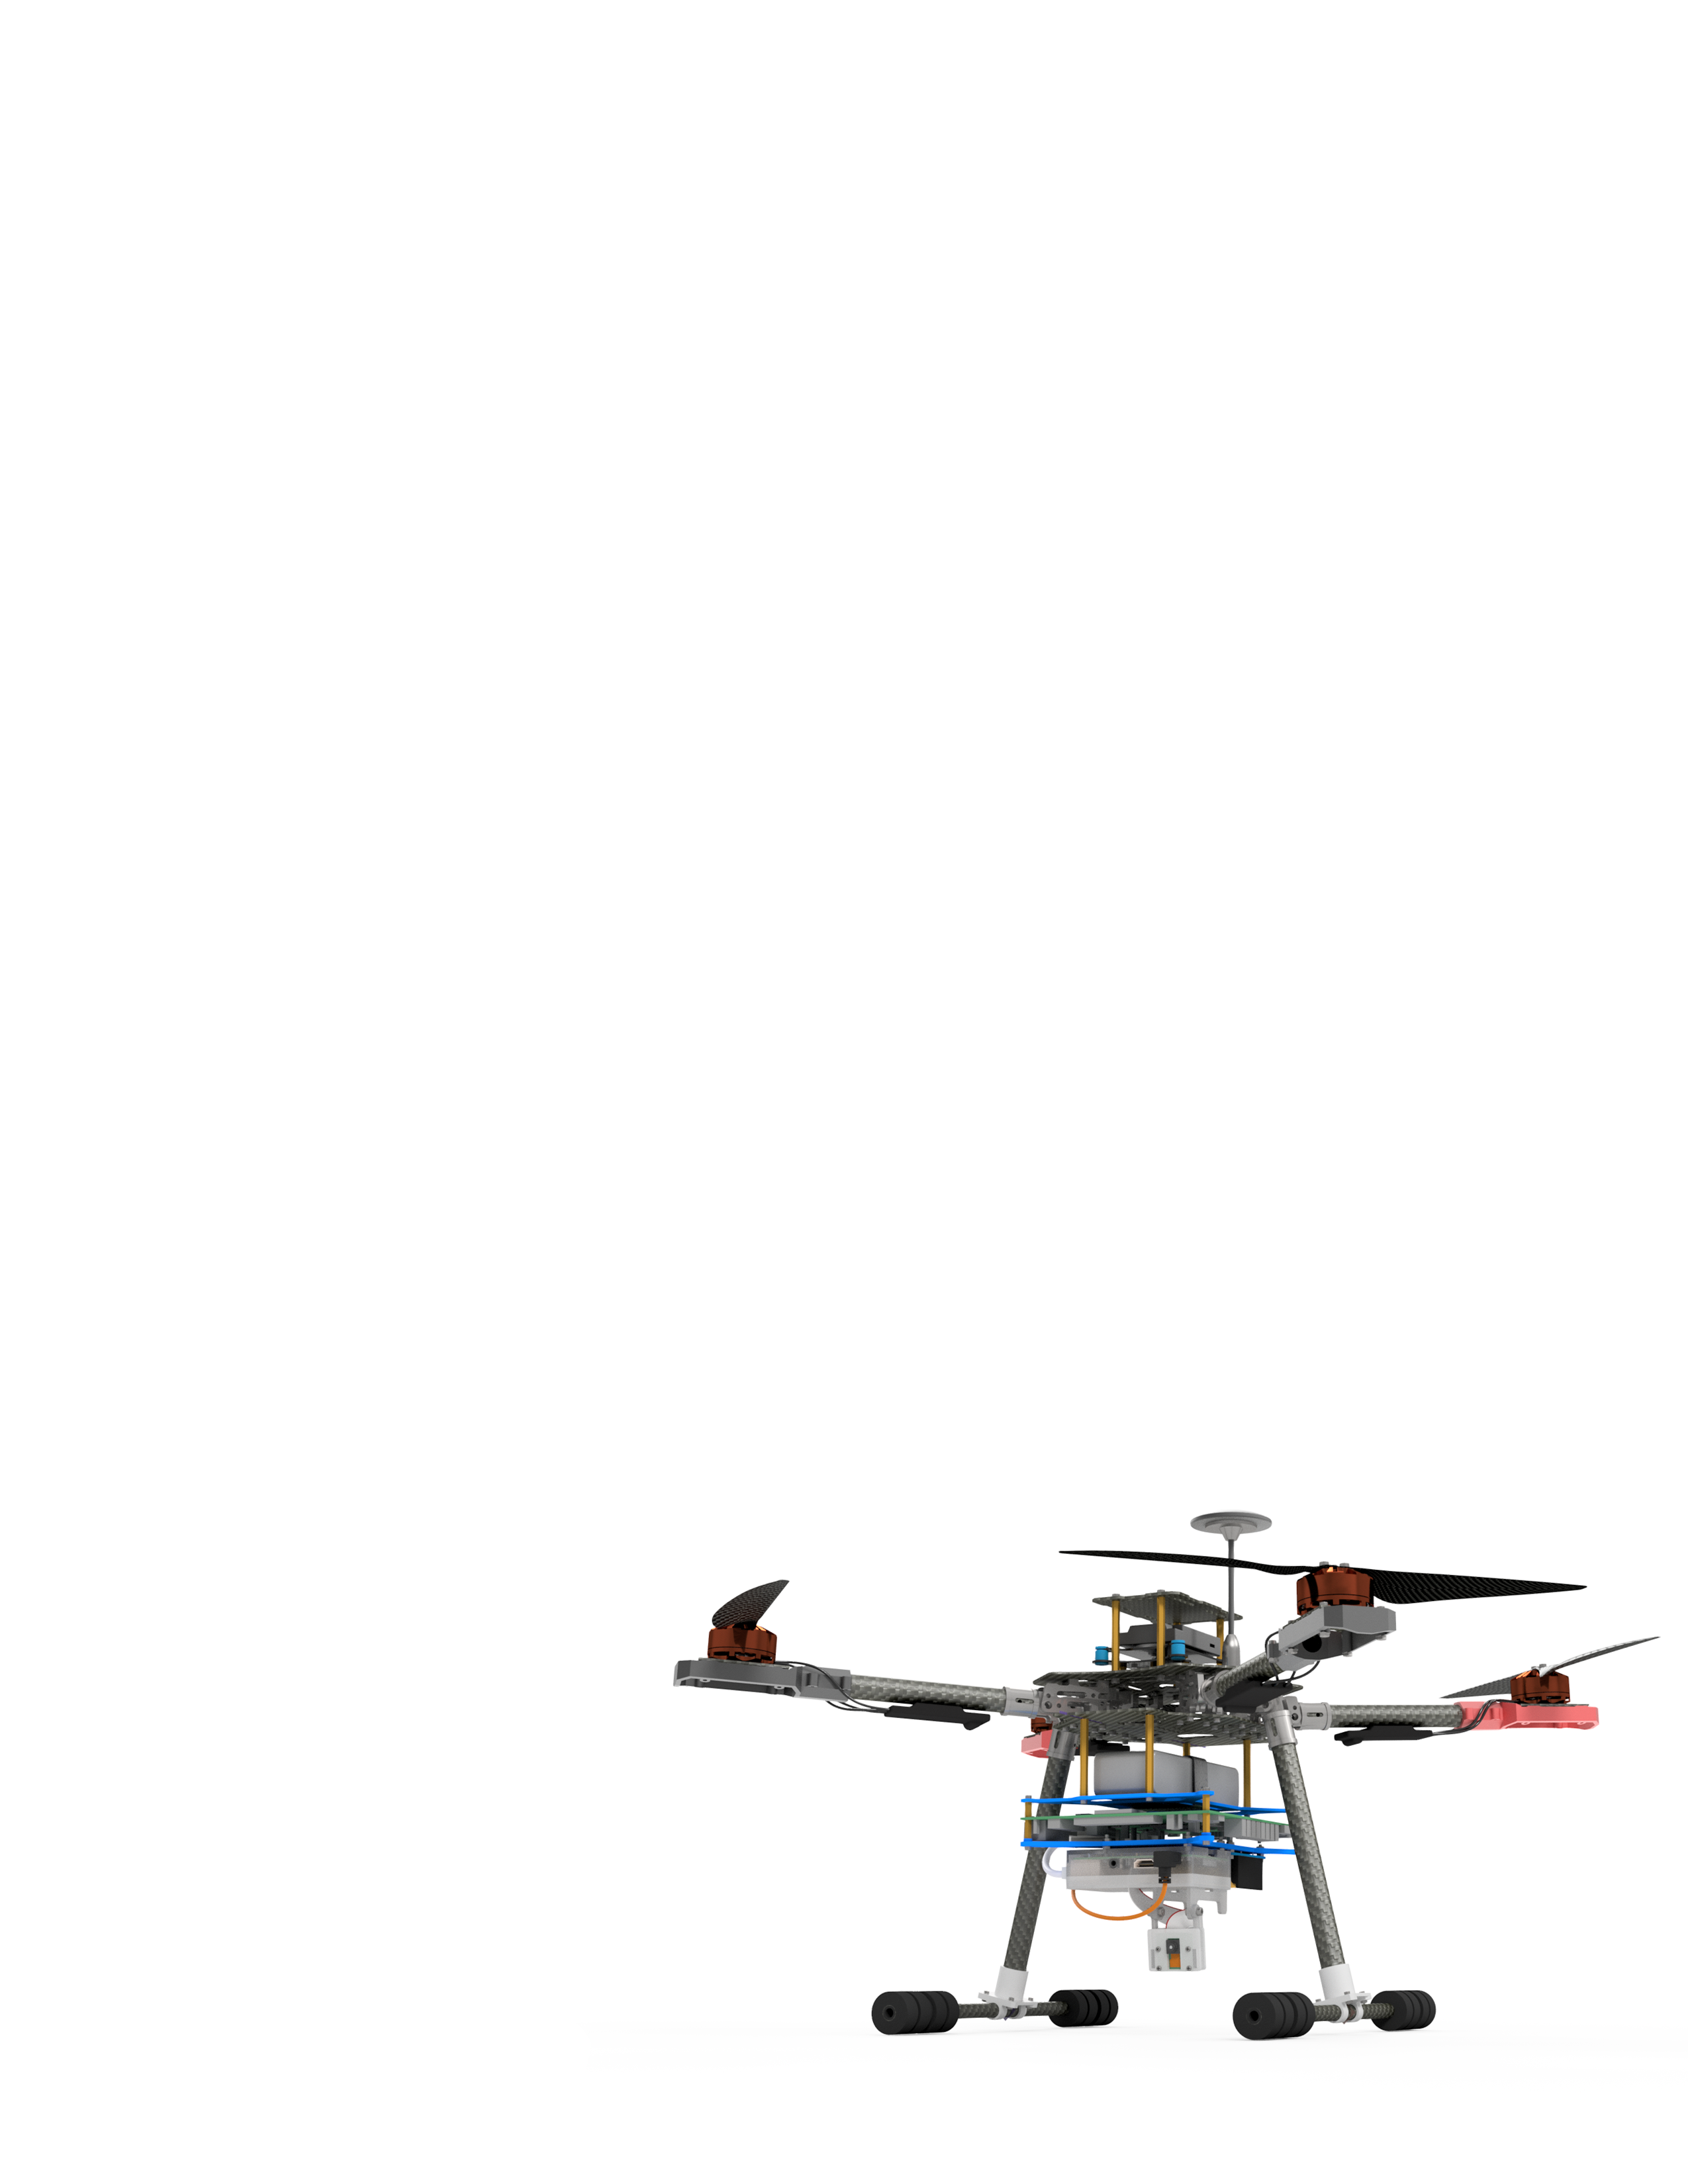
\includegraphics[height=\paperheight,width=\paperwidth]{../assets/render2bg}}
}
\BgThispage
%\thispagestyle{empty}
\section*{Revision History}
The full revision history and commited changes of the document can be found in the git repository history: \href{https://github.com/Capstone-Skynet/Capstone-Skynet.github.io}{https://github.com/Capstone-Skynet/Capstone-Skynet.github.io/commits/master}.

\begin{table}[H]
\begin{tabular}{*{4}{l}p{0.5\linewidth}}
\hline
Version \# & Initials & Release Date & Changeset & Changes Made \\ \hline

0.0 & PD & 2019-10-11 & \texttt{660e001} & Initial skeleton of the document.\\
0.1 & MH & 2019-10-11 & \texttt{6af9e8a} & Populate initial document with draft content required for Milestone I.\\
0.2 & PD & 2019-11-23 & & Initial framework for test descriptions created.\\
0.3 & MW & 2019-11-24 & & First set of tests added.\\
1.0 & PD & 2019-11-25 & & General clean-up and release for Milestone II.\\
1.1 & AH & 2020-02-09 & & Added Full System Tests \\

 & & & \\ \hline
\end{tabular}
\end{table}
\clearpage

% Table of contents
\setcounter{secnumdepth}{3}
\tableofcontents

% Roman numeral page numbers


% Terms and Abbreviations
\thispagestyle{empty}

\section*{Terms and Abbreviations}

Technical terms and abbreviations dictionary go here.

\begin{tabular}[h]{rp{0.75\linewidth}}
    \hline
    \textbf{Term} & \textbf{Definition}\\
    \hline

    ANN & Artificial Neural Network, or simply ``Neural Network'', is a data processing model modeled after neuron interactions. The process consists of forward propagation using several matrix multiplications.\cite{ann}\\
    ASIC & Application-specific Integrated Circuits.\\
    CNN & Convolutional neural network are neural networks that is especially useful for image classification.\cite{cnn} \\
    ECE & Department of Electrical and Computer Engineering at the University of British Columbia.\\
    FPGA & Field-Programmable-Gate-Arrays, ``programmable'' hardware that allows ASIC-like performance with software-like turn-around time and flexibility.\\
    GPU & Graphics Processing Unit, a discrete piece of hardware designed to accelerate graphic-intensive or other parallel computing tasks.\\
    LOS & Line-of-sight.\\
    ML & Machine learning.\\
    Multirotor & An unmanned vehicle with multiple engines. \\
    OTS & Off-the-shelf, or commercially available/purchasable \\
    PID / PID Controller & Proportion-Integral-Derivative controllers is the most common control algorithm for precise and accurate movement, as well as to compensate external forces.\cite{pid}\\
    RNN & Recurrent neural networks are neural networks where the output depends on previous computations, essentially consists of memory.\cite{rnn}\\
    RX & Receiver.\\
    TC & Transport Canada.\\
    TX & Transmitter.\\
    YOLO & You-Only-Look-Once is a fast ML algorithm that detect objects but is unlike CNN nor RNN.\cite{yolo}\cite{yolo-2}\\
     & \\

    \hline

\end{tabular}


% List of figures and tables
\iftotalfigures
\addcontentsline{toc}{section}{\listfigurename}
\listoffigures
\fi
\iftotaltables
\addcontentsline{toc}{section}{\listtablename}
\listoftables
\fi

\newpage

% Set page and section counter
\renewcommand{\thepage}{\arabic{page}}
\setcounter{page}{1}

% TODO: fill out all the sections
% if the sections gets too long, move them to a separte .tex document
\section{About This Document}

\subsection{Purpose}
This document serves to outline the tasks and scenarios likely to be encountered by the client after project delivery. This includes instructions to assemble/build the device, details of maintenance/troubleshooting procedures, and useful tips and tricks. 

\subsection{Intended Audience}
This document is intended for:
\begin{itemize}
\item \textbf{Client (and their representatives)}: to execute steps required for the operation and maintenance of the device,
\item \textbf{Designers (the Capstone team)}: to serve as a central repository of implementation knowledge,
\item \textbf{and Legal Personnel:} to review the installation and maintenance schemes, if necessary. Such personnel may include individuals from the Department of Electrical and Computer Engineering, Industry Canada, and Transport Canada.
\end{itemize}

This document is additionally relevant to those who will assess the maintenance and installation methodology against academic, organizational, or legal criteria.

\subsection{Reading Guide}
This document outlines the following areas of importance to the client: 
\begin{itemize}
\item \textbf{Installation Instructions}: Instructions relating to the construction of the multirotor and computing platform, in addition to how to build/install computing software.
\item \textbf{Flight Checklists}: Instructions relating to the in-flight operation of the computing platform and multirotor.
\item \textbf{Regular Maintenance}: An outline of the maintenance tasks to be taken on the multirotor at predetermined intervals.
\item \textbf{Frequently Asked Questions (FAQs)}: An outline of common questions and answers regarding key points across the entire project.
\item \textbf{Troubleshooting}: A summary of commonly encountered issues with the multirotor and computing platform (and their solutions).
\item \textbf{Suggested Upgrades}: An outline of potential upgrades to the computing platform and multirotor assembly.
\end{itemize}

\clearpage
\section{Installation Instructions}

% TODO: also incorporate drone
\subsection{Computation Platform Hardware Assembly}
The following section outlines the steps required to assemble the computing platform hardware components.

\paragraph{Required Materials}
\begin{itemize}
\item 1 - Zedboard
\item 1 - 12V-12V Barrel Plug Power Adapter (for Zedboard)
\item 1 - Raspberry Pi 4
\item 1 - USB-C to USB-A Cable (for Raspberry Pi)
\item 1 - Raspberry Pi Camera Module
\item 1 - Battery Pack
\item 1 - Battery Pack Charger
\item 1 - Slim Ethernet Cable (1 ft)
\end{itemize}

\paragraph{Instructions}
\begin{enumerate}
\item Ensure that the battery pack is fully charged (as shown by a green status LED indication).
\item Connect the Raspberry Pi and Zedboard to the battery pack using their appropriate power cables (USB-C/USB-A and Barrel/Barrel, respectively).
\item Connect the camera module to the MIPI port on-board the Raspberry Pi, near the headphone jack (taking care not to damage the ribbon cable).
\item Connect the Raspberry Pi and Zedboard with the Ethernet cable.
\end{enumerate}




\subsection{Computation Platform Hardware as Payload Assembly}
% TODO

\subsection{Multirotor Assembly}
% TODO



\subsection{PLB SW/HW Build Instructions}
\label{plb_setup}
The following section outlines the steps required to upload the ML FPGA design, deploy the HPS software environment, and communicate with the PLB through a serial connection.

\paragraph{Required Materials}
\begin{itemize}
\item 1 - Linux/Unix PC with the PetaLinux SDK\cite{petalinux} installed
\item 1 - SD card (at least 4GB in size) \& SD Card Reader
\item 1 - Zedboard \& Power Supply
\item 1 - Micro USB Cable
\end{itemize}

\paragraph{Instructions}
\begin{enumerate}
\item Download (or pull) the latest version of the Capstone-Skynet suite from GitHub (\url{https://github.com/Capstone-Skynet/Integration}).
\item Navigate into the \texttt{Zedboard/yolov2/} folder. 
\item Before continuing, ensure that the PetaLinux settings script has previously been sourced\\ (\texttt{source /opt/pkg/petalinux/settings.sh}, if PetaLinux is installed in its default directory).
\item Pertinent Linux distribution settings have been pre-configured, however if additional configuration is desired (such as including/removing drivers), call \texttt{petalinux-config -c kernel}.
\item Build the project by calling \texttt{petalinux-build}.
\item Prepare the project for the SD card by calling \texttt{petalinux-package -{}-boot -{}-fsbl images/linux/zynq\_fsbl.elf -{}-fpga -{}-u-boot -{}-force}.
\item After inserting the SD card into the reader, determine its disk identifier (\texttt{sudo fdisk -l}). In the next steps, it is assumed that the identifier is \texttt{/dev/sdb}.
\item Open fdisk (\texttt{sudo fdisk /dev/sdb}).
\item Make a new partition by pressing \texttt{n} and make it primary by pressing \texttt{p}.
\item Continue following the fdisk prompts, using the default partition number/first sector, and set the last sector value to be \texttt{+1G} (creating a partition one gigabyte in size).
\item Make the newly created partition bootable by pressing \texttt{a}.
\item Create another partition by pressing \texttt{n} and make it primary by pressing \texttt{p}.
\item Continue following the fdisk prompts, using the default values (the partition will consume the rest of the free space on the SD card).
\item Press \texttt{w} to write the changes to the disk, then exit.
\item Format the first (boot) partition using the FAT format (\texttt{sudo mkfs.vfat -F 32 -n boot /dev/sdb1}).
\item Format the second (root) partition using the EXT4 format (\texttt{sudo mkfs.ext4 -L root /dev/sdb2}).
\item Copy the FPGA initialization file (\texttt{BOOT.BIN}) and Linux micro-boot file (\texttt{image.ub}) to the boot partition (\texttt{sudo cp [BOOT.BIN/image.ub] /media/user/boot/}).
\item Copy the compressed Linux image (\texttt{rootfs.tar.gz}) into the root partition (\texttt{sudo cp rootfs.tar.gz /media/user/root/}). 
\item Navigate to the root partition and extract the compressed image to the base directory (\texttt{sudo tar xvf rootfs.tar.gz}).
\item Extract the weights file found in the \texttt{Zedboard\/} repository directory ( \texttt{yolo\_weights.tar.gz} ) into the home directory of the root user on the SD card.
\item Eject the SD card and insert it into the Zedboard.
\item Ensure that the Zedboard configuration jumpers are set for SD card boot (MI04/MI05 set to 3.3V, remaining to GND).
\item Connect the Zedboard to the PC using the micro USB cable (through the JTAG port), connect the power supply, and switch the Zedboard on.
\item Using PuTTY (or another serial program such as Minicom), open a serial connection to the Zedboard (115200 baud, 8 data bits, 1 stop bit).
\item At the \texttt{Zynq>>} prompt, enter \texttt{boot}.
\item Once Linux boots, use the default root username/password (\texttt{root/root}).
\item Edit the /etc/network/interfaces file to set-up a standard IP configuration for the ethernet adapter. The suggested static IP is \texttt{192.168.1.10} (all scripts are pre-configured to use this).
\end{enumerate}

Once the above steps have been completed, the user can navigate the Linux OS as required. The default program to communicate with the hardware accelerator can be called by entering \texttt{mlprog} at the prompt.

\subsection{PMB SW Build Instructions}
The following section outlines the steps required to install the requisite PMB software onto a Raspberry Pi.

\paragraph{Required Materials}
\begin{itemize}
\item 1 - Raspberry Pi 4 (or above)
\item 1 - Micro-SD card (at least 4GB in size) \& Micro-SD Card Reader
\item 1 - USB-C Power Supply
\end{itemize}

\paragraph{Instructions}
\begin{enumerate}
\item Download and install Raspbian onto a SD card as per standard installation procedures (\url{https://www.raspberrypi.org/documentation/installation/installing-images/})
\item Obtain a Raspbian terminal prompt through any method of choice. One can connect a keyboard/monitor, or SSH can be used to work remotely (\url{https://www.raspberrypi.org/documentation/remote-access/ssh/}).
\item After connecting to the internet, clone the latest version of the Capstone-Skynet suite from GitHub (\url{https://github.com/Capstone-Skynet/Integration})
\item Navigate to the \texttt{RaspberryPi/} folder.
\item Install Python 3, OpenCV-2, and RasPiCam (\url{https://github.com/cedricve/raspicam}) through the linux command prompt (\texttt{apt-get install}). 
\item Install the \texttt{picamera} and \texttt{socketio} python libraries using pip3.
\item Build the C++ helper program \texttt{mlprog} by issuing the following command: \texttt{g++ ml\_server.cpp \-o ml\_server \-I/usr/local/include \-lraspicam \-I/usr/local/include/opencv2 \-L/usr/local/lib/ \-lopencv\_core \-lopencv\_imgproc \-lopencv\_highgui \-lopencv\_ml \-lopencv\_video \-lopencv\_features2d \-lopencv\_calib3d \-lopencv\_objdetect \-lopencv\_contrib \-lopencv\_legacy \-lopencv\_ stitching}
\item Configure the WiFi to connect to the base station network. If working with the command line, this can be done by using the \texttt{sudo raspi-config} command.
\item Edit the /etc/network/interfaces file to set-up a standard IP configuration for the ethernet adapter. The suggested static IP for Ethernet is \texttt{192.168.1.11}  (all scripts are pre-configured to use this).
\item (Optional) Configure the Raspberry Pi to launch the ML suite launch script \texttt{LAUNCH\_ML.sh} automatically on boot using cron (\url{https://www.raspberrypi.org/documentation/linux/usage/cron.md}).
\end{enumerate}

Once the above steps have been completed, the PMB is fully configured.

\subsection{Base Station Configuration Instructions}
\label{bs_inst}
The following section outlines the steps required to configure the Base Station. 

\paragraph{Required Materials}
\begin{itemize}
\item 1 - Device to be used as a server (Windows/Mac/Linux device)
\item 1 - (Optional) Wireless Router
\end{itemize}

\paragraph{Instructions}
\begin{enumerate}
\item \textbf{If using a wireless router}, set the router up by following the manufacturer's instructions and connect the server device to it.

\textbf{If not using a wireless router}, configure the server device to act as a \textit{mobile hotspot}. Consult your operating system vendor for more information.
\item Install Node.js on the server device (\url{https://nodejs.org/en/download/}).
\item Install the \texttt{express} and \texttt{socket.io} Node libraries (\texttt{npm install express; npm install --save socket.io}).
\item Navigate to the \texttt{SkynetWebApp} folder and launch the Node server (\texttt{node server}). 
\item \textbf{On the PMB}, modify the python client (\texttt{PythonClient/pythonclient.py}) to reflect the server's current IP address (this can be found through use of \texttt{ifconfig/ipconfig}).
\end{enumerate}

% TODO: add item to how to get to the web app

Once the above steps have been completed, the base station is fully configured. One can now connect to the web-app by entering the previously determined IP address into the web browser of any device connected to the network. On the server device, one can also navigate to \texttt{localhost} to arrive at the same page.

\subsection{Autopilot Configuration Instructions}
While not necessary for general operations, the client may wish to utilize the autopilot functionality present on the multicopter's on-board control board (separate from the general computational platform where video is captured and machine learning is performed).

% TODO: Split into firmware installation instruction vs using the autopilot configurator

\paragraph{Required Materials}
\begin{itemize}
\item 1 - Windows/Mac/Linux user device to upload/program flight controller firmware
\item 1 - Flight Controller
\item 1 - Micro-USB to USB-A Cable
\end{itemize}

\paragraph{Instructions}

\begin{enumerate}
\item Download and install APM Planner 2.0 (\url{https://ardupilot.org/planner2/}) onto the user device.
\item Download the APM v2.8 firmware (\url{https://ardupilot.org/copter/docs/common-downloads_firmware.html}). Note that v2.8 \textit{must} be used --- the selected control board is not compatible with later versions.
\item Plug the control board into the user device and open APM Planner.
\item Select the control board's relevant COM port and set the baud rate to 115200 (\textit{do not press connect}).
\item Click on \texttt{Initial Setup}, then \texttt{Install Firmware}.
\item Click on the small 'copter' icon, then install the APM v2.8 firmware (previously downloaded).
\item Click \texttt{Connect}
\end{enumerate}


\section{Flight Operations}
The following guides provide calibration steps which may be taken by the user to improve in-flight performance.

\subsection{Pitch and Roll Calibration}
These steps can be followed if the default pitch and roll behaviour of the multicopter during flight is suboptimal.

\paragraph{Required Materials}
\begin{itemize}
    \item 1 - Windows/Mac/Linux user device (with APM planner installed) to program the flight controller 
\item 1 - Flight Controller
\item 1 - Micro-USB to USB-A Cable
\end{itemize}

\paragraph{Instructions}
\begin{enumerate}
	\item Plug the control board into the user device and open APM Planner.
    \item In APM planner, click on the configuration icon, then the advanced parameters tab, and navigate to the \texttt{Logbitmask} section. 
    \item Select \texttt{Default+IMU} from the dropdown menu, then click \texttt{write parameters} in order to enable changes to pitch and roll calibration values during flight.
    \item Click on \texttt{arducopter config}. Set the CH6 opt to \texttt{CH6\_RATE\_KP} using the drop down menu. Set the min to 0.08 and max to 0.15. Disconnect the controller.
    \item Fly the multicopter, adjusting the CH6 knob to adjust the pitch and roll setting of the multicopter to the user's liking. 
    \item After the flight, plug the flight controller back in and re-open APM planner. 
    \item Click on \texttt{Refresh Parameters} to see the optimal pitch/roll value found during flight (it will appear under the P section of \texttt{Rate Roll}. 
    \item To set this value as default, set \texttt{CH6 Opt} to \texttt{CH6\_0None} and click on \texttt{Write Parameters}.
    \item Reset \texttt{Logbitmask} to \texttt{Default} once you are done with configuration.

\end{enumerate}

\subsection{Hover Thrust Configuration}

This test can be performed to update the hover throttle setting to an adjusted value after an initial test flight.

\paragraph{Required Materials}
\begin{itemize}
    \item 1 - Windows/Mac/Linux user device (with APM planner installed) to program the flight controller 
\item 1 - Flight Controller
\item 1 - Micro-USB to USB-A Cable
\end{itemize}

\paragraph{Instructions}
\begin{enumerate}
    \item Plug the control board into the user device and open APM Planner.
    \item In APM Planner, click on \texttt{terminal} and then \texttt{log download}. 
    \item Check the box labeled \texttt{1} and then \texttt{download this log}. 
    \item Click on \texttt{log browse and find the log from the test flight}. 
    \item Scroll down the list and find the row labeled \texttt{CTUN}. Select the entry in the \texttt{throttle in} column and click on \texttt{graph this data}.
    \item Looking at the graph, find the value of the throttle at which the multicopter appears to be at a stable hover.
    \item Return to the \texttt{advanced parameters} configuration screen and change the row labeled \texttt{throttle mid} to the hover value you found in the last section. 
    \item Click on \texttt{write parameters} to complete the update.

\end{enumerate}

\clearpage
\section{Flight Procedures and Checklists}
% Checklist template from
% https://github.com/mavcunha/checklists

% creates empty checkboxes to be used as the second
% argument to \item on checklist
\newcommand{\checkbox}{\makebox[3ex][r]{\Large{$\square$}}}

% checklist env sets up a table and format the items.
% in case a item has steps use the \step{asdf}
% command.
\newenvironment{checklist}[1]{%
  \renewcommand{\item}[2]{%
    ##1\dotfill\makebox{\uppercase{##2}}\\
  }
  \newcommand{\step}[1]{%
    \hspace*{10em}-\hspace*{\labelsep}##1\\
  }
  \begin{tabular}{p{0.9\linewidth}}
     \toprule
       \multicolumn{1}{c}{\textbf{\uppercase{#1}}}\\
     \midrule
}{\bottomrule\end{tabular}\vspace{1em}}


\subsection{Procedures}

\textbf{Computation System Initialization}
\begin{enumerate}
\item Start the web-app server on the Base Station (\texttt{node server}) and connect to the web-app using a web browser (as described in Section \ref{bs_inst}).
\item Turn on the Raspberry Pi by plugging it into the battery pack. Ensure that the red power LED lights up.
\item Turn on the Zedboard using the on-board power switch. Ensure that the power LED (green) and LD1-2 LED (bright blue) light up.
\item If auto-start was not previously configured, connect to the Raspberry Pi via SSH, navigate to the \texttt{Raspberry Pi} folder, and launch the ML suite (\texttt{source LAUNCH\_ML.sh}). Inspect the console for any errors.
\item Examine the web-app. Video should be streaming to the device, and bounding box information should begin to be displayed. Ensure that there are no errors in the web-app's log box.
\end{enumerate}

\textbf{Flight Controller Initialization}
\textit{Note: this checklist is performed automatically by the on-board flight controller -- no user input is required. It is included for user reference only.}
\begin{enumerate}
\item Is the input voltage within nominal range?
\item Is the radio calibrated to the correct operating frequency?
\item Is the accelerometer operational? Has it been calibrated?
\item Is the compass operational? Has it been calibrated?
\item Is the barometer operational?
\item Has a GPS lock been established?
\end{enumerate}

\textbf{Motor Arming}
\begin{enumerate}
	\item Turn on the handheld radio transmitter.
	\item Ensure that the multicopter is in a flat, open area.
	\item Plug in the multicopter's battery. The red and blue lights on the controller will flash momentarily as the gyroscopes are calibrated (do not move the multicopter while this is occuring).
	\item If any initialization failures occur, the LEDs on the controller will indicate an error (see Ardupilot website for specific error details).
	\item Arm the motors by holding the throttle to low, and push the rudder right for 5 seconds. Do not hold the rudder right for more than 15 seconds, otherwise the autotrim feature will be enabled.
	\item Once armed, the LEDs on the controller will stop flashing and the propellors will begin to spin.
	\item Raise the throttle to take off.
\end{enumerate}

\clearpage
\subsection{Checklists}
\begin{multicols}{2}

\begin{checklist}{Before Multirotor Power On}
	\item{Walk-around}{Check}
	Ensure that multirotor is in a flat and open area, far way from bystanders with large safety margin.\\\\
	\item{Airspace}{Check}
	Make sure that the multirotor is not taking off within a controlled airspace.\\\\
	\item{Weather}{check}
	\item{Propellers}{Attached and secured}
	\item{Radio TX}{on}
	\item{Radio TX model}{set}
	\item{Radio TX knobs and switches}{reset}
\end{checklist}

\begin{checklist}{Multirotor Power On}
	\item{Battery}{Charged}Battery voltage at least 11.1 V.\\\\
	\item{Radio TX}{on}
	\item{GPS antenna}{extended}
	\item{Computation platform}{on}
	\item{Battery}{connected}
	\item{Battery balance lead}{connected} Connected battery lead wires to the receiver battery monitoring pins for battery level telemetry on the radio TX.\\\\
\end{checklist}

\begin{checklist}{After Multirotor Power On}
	\item{Autopilot gyroscope}{calibrated}
	\item{Compass}{calibrated}
	\item{GPS lock}{set} Note: this is only applicable for outdoor flights.\\\\
	\item{Autopilot LED}{blue}
	\item{Radio TX RSSI}{on and nominal}
	\item{Radio battery telemetry}{on and nominal}
\end{checklist}

\begin{checklist}{Before Takeoff}
	\item{Computation platform}{online}
	\item{Motors}{armed}
	\item{FCU LED}{red}
\end{checklist}

\begin{checklist}{After Takeoff}
	\item{Flight mode}{set and check}
	\item{Throttle trim}{set for hover at 50\%}
	\item{Roll/pitch/yaw trim}{set}
\end{checklist}

\begin{checklist}{During flight}
	\item{Battery level}{Nominal}
	\item{Radio TX RSSI}{within range}
	\item{Computation platform connection}{nominal}
\end{checklist}

\begin{checklist}{Descent}
	\item{Flight mode}{set to stablize or RTL}
	\item{Roll/pitch/yaw trim}{set}
	\item{Throttle trim}{reset}
\end{checklist}

\begin{checklist}{Before Landing}
	\item{Flight mode}{set to stablize or RTL}
	\item{Landing area}{clear of obstacle}
	\item{Recommended descent rate}{0.2 m/s}
\end{checklist}

\begin{checklist}{After Landing}
	\item{Motors}{disarmed}
	\item{FCU LED}{blue}
\end{checklist}

\begin{checklist}{Multirotor Power Off}
	\item{Battery level}{check}
	\item{Battery}{disconnected}
	\item{Computation platform}{switch off}
	\item{Propellers}{detach}
\end{checklist}

\begin{checklist}{Storage}
	\item{Battery level}{set to 50\%} Charge or discharge the battery to around 50\% to minimize degradation while in storage.\\\\
	\item{Propellers}{detached}
	\item{Cables}{disconnected}
\end{checklist}

\end{multicols}
\clearpage

\section{Regular Maintenance}

% TODO: make a maintenance schedule
% TODO: add battery maintenance tips

To ensure the longevity of the computing platform multirotor, the following maintenance checks should be performed on a regular basis (optimally, prior to every flight session). Failure to rectify issues found during these checks may result in a shortened operational life or danger to the user.

\begin{enumerate}
\item Is the chassis free of mud and dirt?
\item Are there any cracks in the chassis or landing gear? Even small cracks can cause structural failure.
\item Are all screws tightly in place?
\item Are the propellers tightly in place and free of cracks? Are they free-spinning? \textit{Ensure that the battery is disconnected during this check.}
\item Are all wires securely connected and free of fraying?
\item Is the camera clear of obstruction and dirt?
\item Are the antennae straight and properly fitted?
\item Are the batteries (and their chargers) free of visible damage? Are the batteries bulging?
\end{enumerate}

The on-board batteries will degrade in capacity over time, and will need to be replaced with suitable replacements after extended use (see \textit{Validation Specification} for potential upgrades).

Apart from ensuring cleanliness and a lack of physical damage, no particular maintenance must be performed on the computation platform.

\section{FAQs}
\textbf{What are the different programs running on the computation platform?}

There are four programs in total across the PLB, PMB, and base station:

\texttt{mlprog} (C-based) runs on the PLB and controls low-level PLB/acceleration operations.

\texttt{ml\_server} (C++-based) runs on the PMB and controls communications to the PLB (sending images and retrieving results).

\texttt{pythonClient.py} (Python-based) acts as a shim to interface the web-app with the PMB.

\texttt{server} (Node.js-based) acts as the central base-station server and serves the video feed/system status to the end user.

\textbf{Can I test the system without flying the multicopter?}

Yes, the computation platform and the multicopter control platform are independent systems. One can test the machine learning component on the ground, or even substitute pre-recorded 640x480 video into the processing stream (see \texttt{ml\_server.cpp} for more information regarding video-in capabilities).

\textbf{How do I make improvements to the framerate/hardware accelerator?}

While making adjustments to the machine learning accelerator is possible (given that it is HLS-based), such adjustments are outside the scope of the project. One can refer to the original accelerator GitHub page (\url{https://github.com/dhm2013724/yolov2_xilinx_fpga}) for further build/customization information.

\textbf{How do I extend the operational range of the multirotor?}

The prefered route to extend the operational range is to increase the battery capacity of the platform. Refer to the \textit{Validation Specification} for specific battery configuration suggestions.

\section{Troubleshooting}
\textbf{Zedboard and/or Raspberry Pi power lights do not turn on}
\begin{enumerate}
\item Ensure that the battery pack is fully charged.
\item Ensure that the power cables are properly seated.
\end{enumerate}

\textbf{No image is displayed on the web app}
\begin{enumerate}
\item Ensure that the Computation System Initialization checklist has been fully followed.
\item Check that the camera module ribbon cable is properly seated and the cable itself is not damaged.
\item Move multirotor platform closer to the base station to avoid connectivity issues.
\item Restart the ML suite via SSH.
\end{enumerate}

\textbf{LD1-2 LED on Zedboard does not light on boot}
\begin{enumerate}
\item Ensure that the SD card in the Zedboard is properly seated.
\item Ensure that Zedboard HW jumpers are properly set.
\item Re-flash the Zedboard SD card. (\ref{plb_setup}).
\end{enumerate}

\textbf{Socket errors appear in console/logs}
\begin{enumerate}
\item Ensure that the ethernet connection between the Zedboard and the Raspberry Pi is secure and established (the LEDs on each ethernet port should glow green upon a successful link).
\item Ensure that the Raspberry Pi is connected to the Base Station's WiFi network.
\item Ensure that the IP addresses specified in \texttt{pythonClient.py} and \texttt{mlprog.cpp} match those of the corresponding devices.
\end{enumerate}

\clearpage
\section{Suggested Upgrades}
This section outlines potential future upgrades to subsystems which will increase the quality, usability, and reliability of the computing platform multirotor. 

\subsection{Choice of ML Model}
As outlined in the project requirements, the chosen machine learning model is intended to be replaced by the client with their own implementation. This could be another implementation of the YOLOv2 model, a different pre-designed network, or an entirely custom network. While the current machine learning implementation (YOLOv2) is extremely versatile (being able to detect 75+ different classes), such a system may not ultimately be desirable to the client. For instance, if the client later wishes to specialize the system to \textit{only detect pedestrians}, YOLOv2 is likely unnecessarily complex, imposing onerous delays to an otherwise simple detection. If this is the case, the client may wish to adopt a simpler network such as MobileNet or TinyYolo.

\subsection{Existing ML Model Improvements}
If the client decides to improve on the existing machine learning hardware design rather than replace it outright there are several opportunities to improve its performance. Currently the hardware accelerator runs at 50MHz, however with some experimentation (and appropriate timing analysis), it is likely possible to raise the accelerator's clock frequency (and ultimately decrease the end-to-end ML latency). Additional parallelism improvements could also be applied to the AXI interconnect between the HPS and the accelerator, increasing the transfer speed of both the images to the accelerator and the results back to the HPS.

\subsection{Improved WiFi Antenna}
As detailed in the \textit{Design Document}, while the WiFi antenna on-board the Raspberry Pi 4 is sufficient to sustain video streaming at short-to-medium ranges (10-15 metres), the connection quality becomes insufficient at larger distances. During development it was determined that a dedicated USB WiFi card would alleviate these range issues (having better reception than the trace-based antenna on the Raspberry Pi), however this purchase was forgone in light of the COVID-19 pandemic. 

\subsection{Video Encoding and Streaming}
In the current implementation, video captured from the camera is sent to the base station frame-by-frame in JPEG format. The system was designed in such a manner to simplify the development of both the PMB and Base Station, however such a design imposes heavy bandwidth requirements onto the (already weak) WiFi connection. To further improve range and decrease bandwidth requirements, different video encodings (such as H264) could be examined, allowing for the exploitation of frame-to-frame compression.

\subsection{Result Storage and Retrieval}
Due to the COVID-19 pandemic, the video and result retrieval mechanism was not implemented as per the original requirements. While storing ML results is a trivial file I/O exercise, storing videos would require additional video encoding frameworks to be implemented (as previously described). Footage retrieval is another area of difficulty, as the end user should be able to browse and download files directly from the web-app (rather than having to retrieve files through means such as \texttt{scp}), and as such a file server would need to be configured on the PMB.  

% Bibliography
\clearpage
\addcontentsline{toc}{section}{References}
\bibliographystyle{ieeetr}
\bibliography{references}

% Appendix (uncomment to enable appendix)
% \clearpage
% \appendix
% \section{Appendix name}\label{appendix:sample-appendix}
% Content here

\end{document}
